\documentclass[12pt, twoside]{article}
\usepackage[letterpaper, margin=1in, headsep=0.5in]{geometry}
\usepackage[english]{babel}
\usepackage[utf8]{inputenc}
\usepackage{amsmath}
\usepackage{amsfonts}
\usepackage{amssymb}
\usepackage{tikz}
\usetikzlibrary{quotes, angles}
\usepackage{graphicx}
\usepackage{enumitem}
\usepackage{multicol}

\newif\ifmeta
\metatrue %print standards and topics tags

\title{Regents Geometry}
\author{Chris Huson}
\date{September 2020}

\usepackage{fancyhdr}
\pagestyle{fancy}
\fancyhf{}
\renewcommand{\headrulewidth}{0pt} % disable the underline of the header
\raggedbottom


\fancyhead[LE]{\thepage}
\fancyhead[RO]{\thepage \\ Name: \hspace{4cm} \,\\}
\fancyhead[LO]{BECA / Dr. Huson / Geometry 09-Congruence-transformations\\* pset ID: 161}

\begin{document}

\subsubsection*{9-8DN-Similarity-review}
\begin{enumerate}
\item Two triangles are shown with $P$ the intersection of $\overline{AJ}$ and $\overline{BK}$.
  \begin{multicols}{2}
    \begin{enumerate}
        \item Justify $\angle APB \cong \angle JPK$.
        \item What angle must be congruent to $\angle B$ to prove $\triangle ABP \sim \triangle JKP$ by \emph{angle-angle similarity}? \vspace{2cm}
        \end{enumerate}
    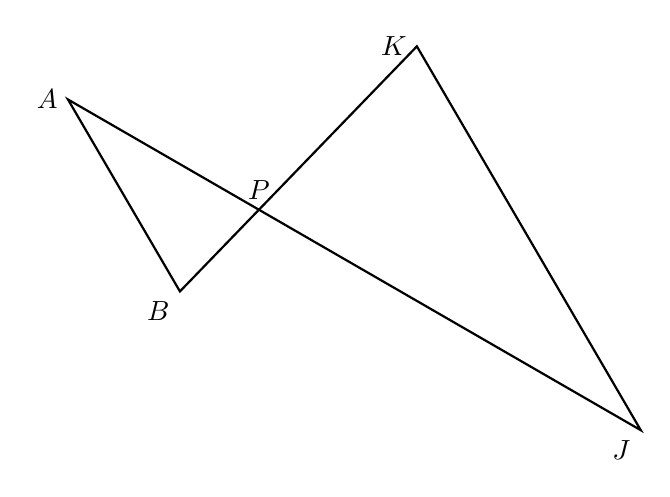
\begin{tikzpicture}[rotate=-30, scale=1.4]
        \draw [thick]
          (-0.25,-1)node[below left]{$B$}--
          (0.5,2)node[left]{$K$}--
          (4,0)node[below left]{$J$}--
          (0,0)node[above]{$P$}--
          (-2,0)node[left]{$A$}--cycle;
      \end{tikzpicture}
    \end{multicols}
      \vspace{1cm}

\item Given $\triangle PQR \sim \triangle STU$, $m\angle P=37^\circ$, and $m\angle T=46^\circ$. Find $m\angle Q$. \vspace{3cm}

\item The diagram below shows $\triangle ABC$, with $\overline{AEB}$ and $\overline{ADC}$.
    \begin{multicols}{2}
      \begin{enumerate}
        \item Justify $\angle BAC \cong \angle DAE$.
        \item What angle must be congruent to $\angle AED$ to prove $\triangle ABC \sim \triangle ADE$ by \emph{angle-angle similarity}? \vspace{3cm}
      \end{enumerate}
      \begin{tikzpicture}[scale=1.3]
        \draw [thick]
        (0,0) node[above right] {$A$}--
        (230:6) node[below left] {$B$}--
        (260:4.75) node[below right] {$C$}--cycle;
        \draw [thick]
        (230:2.375) node[above left] {$E$}--
        (260:3) node[right] {$D$}--cycle;
      \end{tikzpicture}
    \end{multicols}

\newpage
\item A dilation centered at the origin with scale factor $k=\frac{4}{3}$ maps $\overline{AB} \rightarrow \overline{A'B'}$. 
  \begin{multicols}{2}
    \begin{enumerate}
      \item Draw and label the image.
      \item What is the ratio of the length of $\overline{A'B'}$ to $\overline{AB}$?
      \item What is the relationship of the slope of $\overline{A'B'}$ and $\overline{AB}$?
      \begin{flushright}
        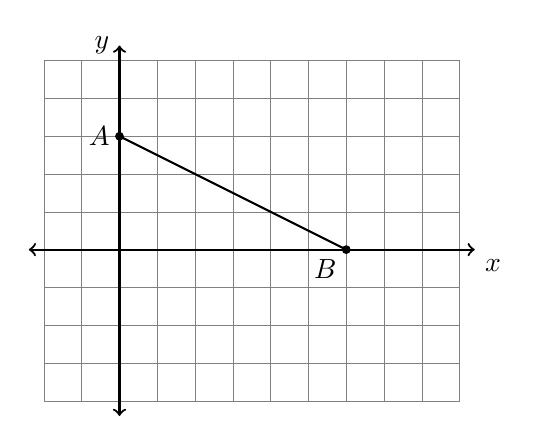
\begin{tikzpicture}[scale=.48]
          \draw [help lines] (-2,-4) grid (9,5);
          \draw [thick, <->] (-2.4,0) -- (9.4,0) node [below right] {$x$};
          \draw [thick, <->] (0,-4.4)--(0,5.4) node [left] {$y$};
          \draw [thick] (0,3)--(6,0);
          \draw [fill] (0,3) circle [radius=0.1] node[left] {$A$};
          \draw [fill] (6,0) circle [radius=0.1] node[below left] {$B$};
        \end{tikzpicture}
      \end{flushright}
    \end{enumerate}
    \end{multicols} \vspace{1cm}
    
\item Given $\triangle ABC$, $D$ is the midpoint of $\overline{BA}$, $E$ is a point on $\overline{BC}$, and $\overline{DE}$ is drawn. \\*[2pt] 
    If $BD=8$ and $BE=10$, what is the length of $\overline{BC}$ so that $\overline{AC} \parallel \overline{DE}$?
    \begin{flushright}
        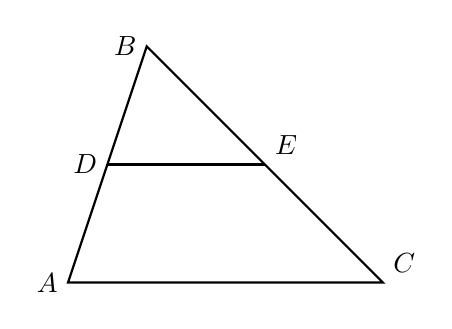
\begin{tikzpicture}[scale=0.5]
          \draw [thick]
          (0,0)node[left]{$A$}--
          (8,0)node[above right]{$C$}--
          (2,6)node[left]{$B$}--cycle;
          \draw [thick]
          (1,3)node[left]{$D$}--
          (5,3)node[above right]{$E$};
        \end{tikzpicture}
      \end{flushright}

\item In diagram below, each centimeter represents six inches. Find the length of each side in feet. (measure with a metric scale)
    \begin{multicols}{2}
      \begin{enumerate}[itemsep=1.5cm]
        \item $AB=$
        \item $BC=$
        \item $AC=$ 
        \item Find the area of $\triangle ABC$
      \end{enumerate}
    \begin{center}
      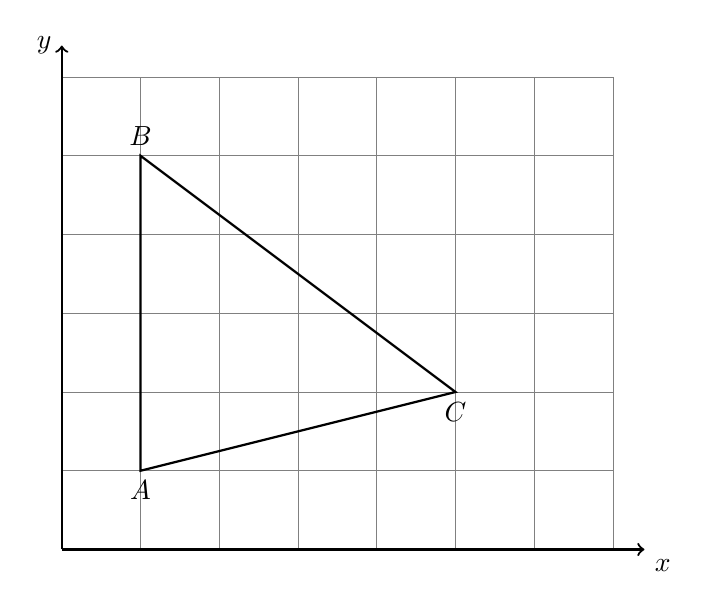
\begin{tikzpicture}
        \draw [help lines] (0,0) grid (7,6);
        \draw [thick, ->] (0,0) -- (7.4,0) node [below right] {$x$};
        \draw [thick, ->] (0,0)--(0,6.4) node [left] {$y$};
        \draw [thick] (1,1)node[below]{$A$}--(5,2)node[below]{$C$}
        --(1,5)node[above]{$B$}--cycle;
      \end{tikzpicture}
    \end{center}
  \end{multicols}%\vspace{2cm}

\newpage
\item Given $\triangle ABP \sim \triangle JKP$ as shown below. $AB=10.0$, $AP=9.0$, $BP=5$, and $AJ=27.0$. Find $JK$.
    \begin{flushright}
    \begin{tikzpicture}[scale=1.4]
        \draw [thick]
          (-0.25,-1)node[below left]{$B$}--
          (0.5,2)node[left]{$K$}--
          (4,0)node[below left]{$J$}--
          (0,0)node[above left]{$P$}--
          (-2,0)node[left]{$A$}--cycle;
      \end{tikzpicture}
      \end{flushright}
      \vspace{0.5cm}

\item The vertices of $\triangle JKL$ have the coordinates $J(-4,-2)$, $K(3,2)$, and $L(-2,4)$, as shown. \\[0.25cm]
    Apply a dilation to $\triangle JKL \rightarrow \triangle J'K'L'$, centered at $P(-1,2)$ and with a scale factor $k=2$. Draw the image $\triangle J'K'L'$ on the set of axes below, labeling the vertices, and make a table showing the correspondence of both triangles' coordinate pairs.
      \begin{flushright}
        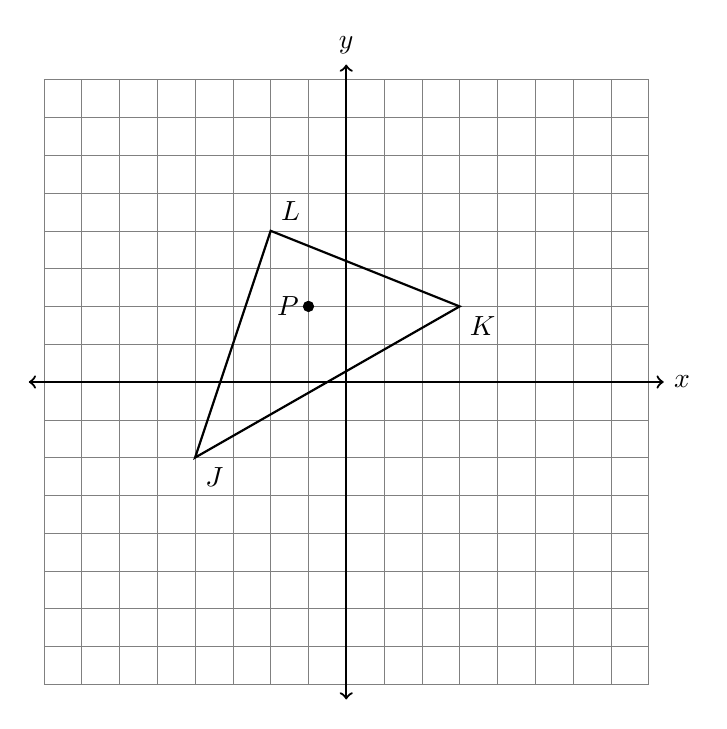
\begin{tikzpicture}[scale=.48]
          \draw [help lines] (-8,-8) grid (8,8);
          \draw [thick, <->] (-8.4,0) -- (8.4,0) node [right] {$x$};
          \draw [thick, <->] (0,-8.4)--(0,8.4) node [above] {$y$};
          \draw [thick]
            (-4,-2) node[below right] {$J$}--
            (3,2) node[below right] {$K$}--
            (-2,4) node[above right] {$L$}--
            cycle;
          \fill (-1,2) circle[radius=0.15cm]node[left]{$P$};
        \end{tikzpicture}
      \end{flushright}
      What is the ratio of the area of $\triangle JKL$ to $\triangle J'K'L'$?

\newpage
\item In $\triangle ABC$ shown below, $\angle ACB$ is a right angle, $E$ is a point on $\overline{AC}$, and $\overline{ED}$ is drawn perpendicular to hypontenuse $\overline{AB}$.
    \begin{center}
      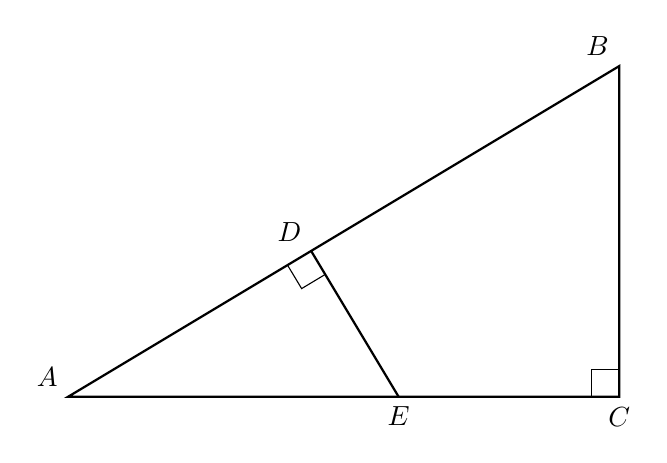
\begin{tikzpicture}[scale=0.7]
        \draw [-, thick] (0,0) node[above left]{$A$}--
        (10,0) node[below]{$C$}--
        (10,6) node[above left]{$B$}--cycle;
        \draw [thick] (6,0)--(4.41,2.65);
        \node at (6,0) [below]{$E$};
        \node at (4.41,2.65) [above left]{$D$};
        \draw (10,0) ++(-0.5,0)--++(0,0.5)--++(0.5,0);
        \draw (4.41,2.65) ++(-59:0.5)--++(-149:0.5)--++(121:0.5);
        %\node at (4, 0) [below]{$12$};
        %\node at (3,2) [above]{$9$};
        %\node at (9, 3) [right]{$10$};
        %\node at (5.5, 1.6) [right]{$6$}; \vspace{1cm}
      \end{tikzpicture}
    \end{center} 
    If $AB = 9$, $BC = 6$, and $DE = 4$, what is the length of $\overline{AE}$? \vspace{3cm}

\item In the diagram below, $\angle ABC \cong \angle ADE$, $AB = 9$, $AC = 6$, $BD = 13.5$, and $DE = 16$. Find  $AD$ and the scale factor $k$. Then find $AE$ and $BC$. %\vspace{1cm}
  \begin{multicols}{2}
    \begin{enumerate}
      \item $AD=$ \vspace{0.3cm}
      \item $k=$ \vspace{0.3cm}
      \item $AE=$ \vspace{0.3cm}
      \item $BC=$
    \end{enumerate}
    \begin{flushright}
      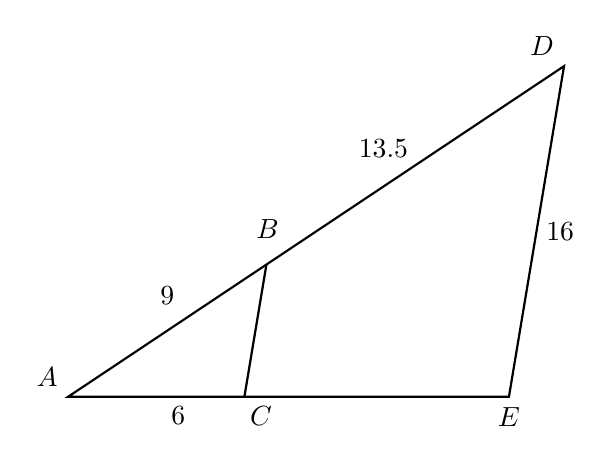
\begin{tikzpicture}[scale=0.7]
        \draw [-, thick] (0,0) node[above left]{$A$}--
        (8,0) node[below]{$E$}--
        (9,6) node[above left]{$D$}--cycle;
        \draw [thick] (3.2,0)--(3.6,2.4);
        \node at (3.5,0) [below]{$C$};
        \node at (4,2.7) [above left]{$B$};
        \node at (2, 0) [below]{$6$};
        \node at (1.8,1.5) [above]{$9$};
        \node at (8.5, 3) [right]{$16$};
        \node at (5.1, 4.5) [right]{$13.5$}; \vspace{1cm}
      \end{tikzpicture}
    \end{flushright} 
  \end{multicols}\vspace{1cm}

\newpage
\item The line $\overleftrightarrow{AB}$ has the equation $y=\frac{2}{3}x-2$. Apply a dilation mapping $\overleftrightarrow{AB} \rightarrow \overleftrightarrow{A'B'}$ with a factor of $k=3$ centered at the origin. Draw and label the image on the grid. Write the equation of the line $\overleftrightarrow{A'B'}$.
    \begin{flushright} %4 quadrant regents grid w T-Chart
    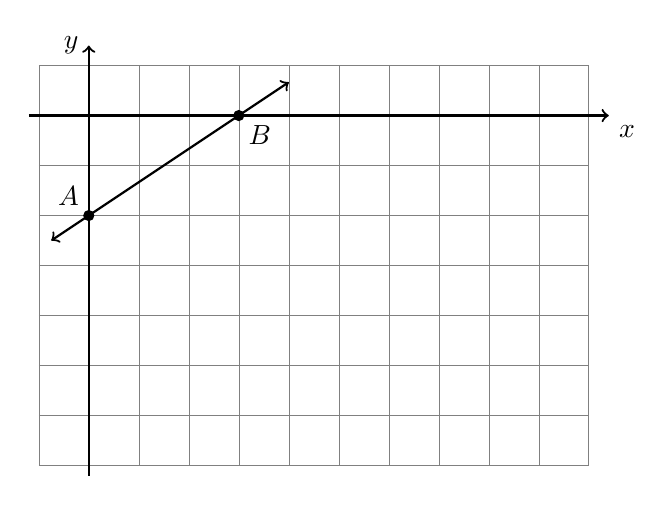
\begin{tikzpicture}[scale=.635]
      \draw [help lines] (-1,-7) grid (10,1);
      \draw [thick, ->] (-1.2,0) -- (10.4,0) node [below right] {$x$};
      \draw [thick, ->] (0,-7.2)--(0,1.4) node [left] {$y$};
      \draw [<->, thick] (-0.75,-2.5)--(4,0.667);
      \draw [fill] (0,-2) circle [radius=0.1]node[above left]{$A$};
      %\draw [fill] (3,0) circle [radius=0.1]node[below left]{$C$};
      \draw [fill] (3,0) circle [radius=0.1]node[below right]{$B$};
    \end{tikzpicture}
    \end{flushright}

\item The diagram below shows $\triangle ABC$. $E$ bisects $\overline{AB}$, and $\angle ACB \cong \angle AED$. $AB=18$, $AC=12$, and $DE=7$. Find the scale factor $k$, $BC$, and $AD$.
  \begin{multicols}{2}
    \begin{enumerate}
      \item $k=$ \vspace{1cm}
      \item $BC=$ \vspace{1cm}
      \item $AD=$  \vspace{1cm}
    \end{enumerate}
      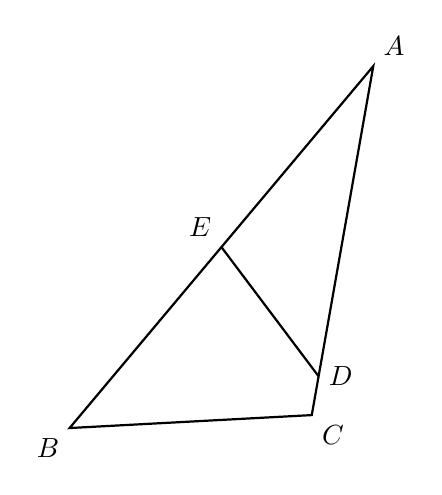
\begin{tikzpicture}[scale=1.0]
        \draw [thick]
        (0,0) node[above right] {$A$}--
        (230:6) node[below left] {$B$}--
        (260:4.5) node[below right] {$C$}--cycle;
        \draw [thick]
        (230:3) node[above left] {$E$}--
        (260:4) node[right] {$D$}--cycle;
      \end{tikzpicture}
    \end{multicols}\vspace{0.5cm}

\item In the diagram below, the chords $\overline{AE}$ and $\overline{BD}$ intersect at $C$. Given $\triangle ABC \sim \triangle DEC$, $BC=6$, $CD=12$, and $CE=10$. Determine the length of $\overline{CA}$.
    \begin{flushright}
    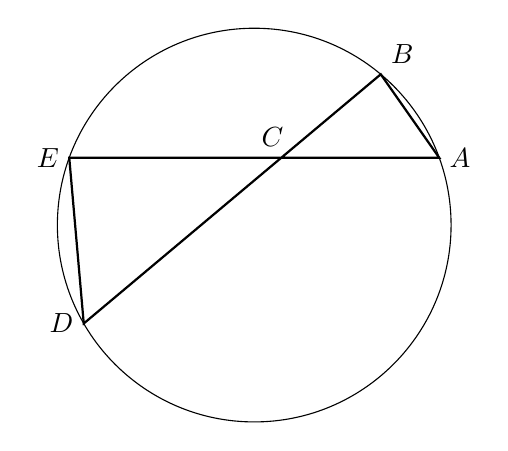
\begin{tikzpicture}[scale=.5]
      \draw (0,0) circle[radius=5];
      \draw [thick]
      (20:5) node[right] {$A$}--
      (160:5) node[left] {$E$}--
      (210:5) node[left] {$D$}--
      (50:5) node[above right] {$B$}--cycle;
      \draw (75:1.8) node[above] {$C$};
    \end{tikzpicture}
  \end{flushright}

\newpage
\item What transformation or series of transformations map $\triangle ABC$ onto $\triangle DEF$, shown below? Fully specify the transformation(s).
  \begin{flushright}
    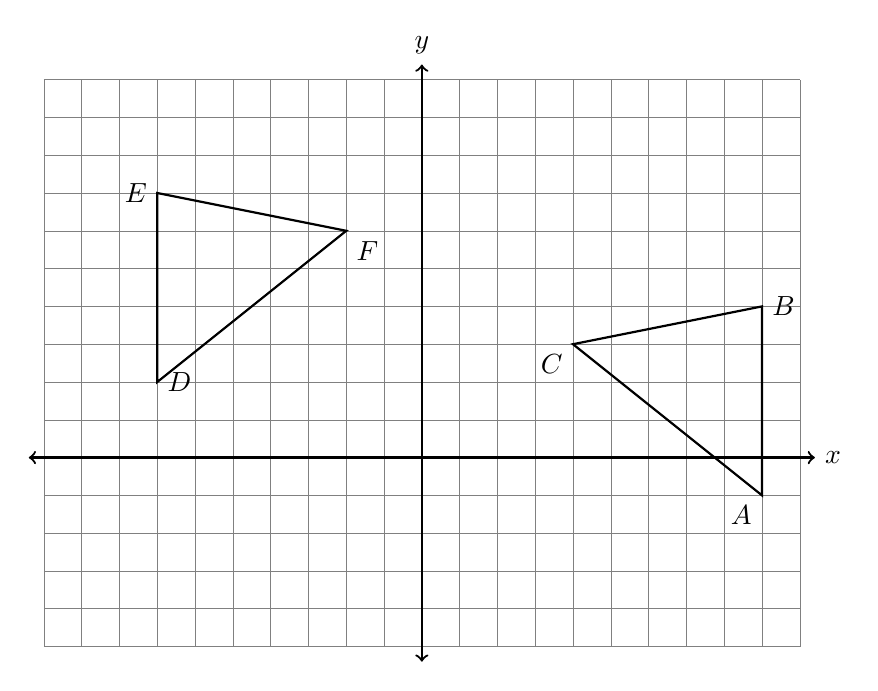
\begin{tikzpicture}[scale=.48]
      \draw [help lines] (-10,-5) grid (10,10);
      \draw [thick, <->] (-10.4,0) -- (10.4,0) node [right] {$x$};
      \draw [thick, <->] (0,-5.4)--(0,10.4) node [above] {$y$};
      \draw [thick]
        (9,-1) node[below left] {$A$}--
        (9,4) node[right] {$B$}--
        (4,3) node[below left] {$C$}--cycle;
      \draw [thick]
        (-7,2) node[right] {$D$}--
        (-7,7) node[left] {$E$}--
        (-2,6) node[below right] {$F$}--cycle;
    \end{tikzpicture}
  \end{flushright}

\item Reflect $\triangle ABC$ over the $y$-axis then dilate the resulting triangle by a factor of 2 centered at the origin.
  \begin{flushright}
  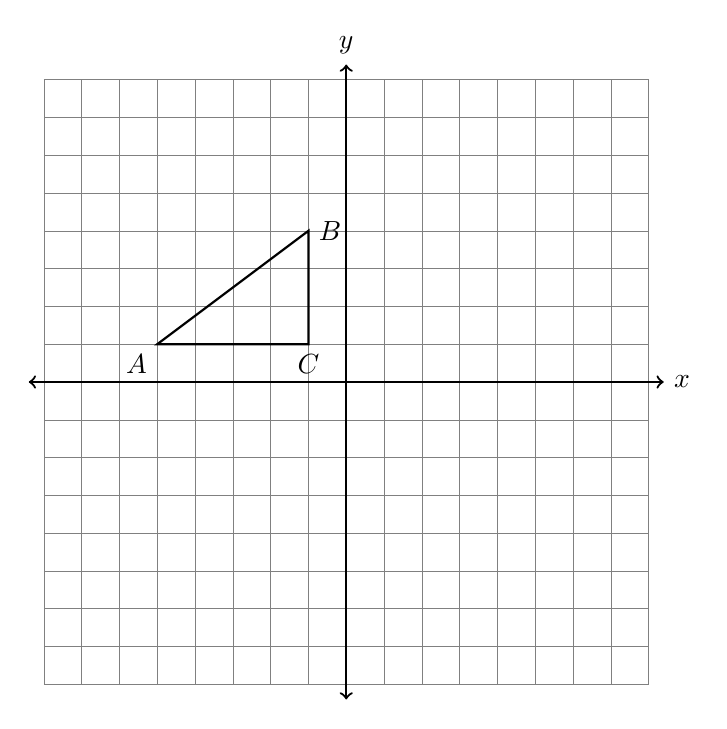
\begin{tikzpicture}[scale=.48]
    \draw [help lines] (-8,-8) grid (8,8);
    \draw [thick, <->] (-8.4,0) -- (8.4,0) node [right] {$x$};
    \draw [thick, <->] (0,-8.4)--(0,8.4) node [above] {$y$};  
    \draw [thick]
      (-5,1) node[below left] {$A$}--
      (-1,4) node[right] {$B$}--
      (-1,1) node[below] {$C$}--cycle;  
  \end{tikzpicture}
  \end{flushright}

\end{enumerate}
\end{document}